
\section{Scene}

In this section we are looking at the structure and behaviour of our implementation of a scene. In order to understand, why we structured our scenes the way we did, we first need to take a look at the glTF file format, from which our scenes are loaded from.

\subsection{glTF Structure}

A glTF file stores its data in the JSON format. There are different types of objects in glTF and each of them is stored in an array. An objects can reference an other object by its index in the respective array. The objects we are interested in are:

\section{Scene}

In this section, we are looking at the structure and behaviour of our scene implementation. In order to understand why we structured our scenes the way we did, we first need to take a look at the glTF file format from which our scenes are loaded.

\subsection{glTF Structure}

A glTF file stores its data in the JSON format. There are different types of objects in glTF, each stored in an array. An object can reference another object by its index in the respective array. The objects we are interested in are:

\begin{itemize}
    \item \textbf{Buffer, Buffer view and Accessor}

    These three objects work together closely. A buffer stores a block of binary data, usually contained in a separate BIN file, and a buffer view describes a specific part of a buffer. A buffer view contains a reference to a buffer and an offset, length, and optional stride. A buffer view sees the data as just raw bytes. To associate some meaning to the data, we use an accessor. It references a buffer view at a particular offset and contains the number of elements, as well as the type (e.g., scalar, vec3, mat4) and component type (e.g., float, unsigned int) of the elements. Accessors can be used for things like vertex attributes and joint matrices.

    \item \textbf{Mesh}

    A mesh stores a static 3D model. It contains a material and an array of primitives. Each primitive has a mode (e.g., points, lines, triangles), an optional accessor for indices, and a set of accessors for the different vertex attributes (e.g., positions, normals, uv coordinates, vertex colors, joint weights).

    \item \textbf{Skin}

    A skin is used for skeletal animation of a mesh. It contains an array of nodes that are used as the skeleton's joints and an accessor for the inverse bind matrices of the joints.

    \item \textbf{Node}

    This represents a node in the scene graph. A node always has a transform, which is either represented by a 4x4 matrix or a scale (vec3), rotation (quaternion), and translation (vec3). A node can have an array of child nodes, which inherit the transform of the parent node. In other words, a node's transform is applied in the parent node's coordinate system.

    A node can optionally also contain a mesh and, if a mesh is present, also a skin. The skin can deform the node's mesh during an animation.

    \item \textbf{Scene}

    A scene contains an array of root nodes. These nodes and all of their children are part of that scene.

    \item \textbf{Animation}

    An animation has an array of channels and an array of samplers. A channel describes which property is being sampled during the animation. It contains the affected node and a path for the node's affected property (e.g., "transform", "scale", "rotation"). It also holds a reference to one of the animation samplers. 

    A sampler calculates a property's value at a certain point in time from a set of key frames. It contains two accessors, one for the time of the key frames and one for the value of the key frames. Additionally, a sampler contains the interpolation type that should be used to sample a value.


\end{itemize}

There are also some other objects (e.g., materials, textures, and cameras), but since they are not relevant to our application, we don't explain them here.

\subsection{Scene Structure}

We will now take a look at the structure of our scene implementation. For this we will look at the C++ classes we used to implement the different glTF objects.


\subsubsection{The \code{Scene} class}

The \code{Scene} class represents a scene loaded from a glTF file. It contains an array of nodes, an array of animations, and an array of skins. Additionally, it stores the TLAS used for ray traversal and the buffers used by the scene in a \code{SceneBuffers} struct.

A scene can be loaded using the static method \code{Scene::load}, which takes the path to the glTF file as a parameter. The class also provides \code{Scene::iter}, which returns an iterator over all nodes in the scene. The function \code{Scene::build\_acceleration\_structures} creates our acceleration structures and must be called when using the scene for ray tracing. Other scene functions are explained in the following subsection on updating a scene (see \autoref{subsec:updating-a-scene}).

\subsubsection{The \code{Mesh} class}

The \code{Mesh} class represents a glTF mesh. It stores an array of \code{Primitive}s. Each \code{Primitive} contains three sub-buffers: \code{positions} for vertex positions, \code{indices} for vertex indices, and \code{joint\_weights} for joint weights used in skinning. The positions and indices store sequences of \code{vec3}s and \code{unsigned int}s, respectively. Joint weights are stored as a 2D array of \code{JointWeight} structs, where each \code{JointWeight} contains the index of a node in the skeleton and its corresponding weight. All joint weights for a vertex are stored sequentially, as shown in Figure~\ref{fig:joint-weights}.

\begin{figure}[H]
    \centering
    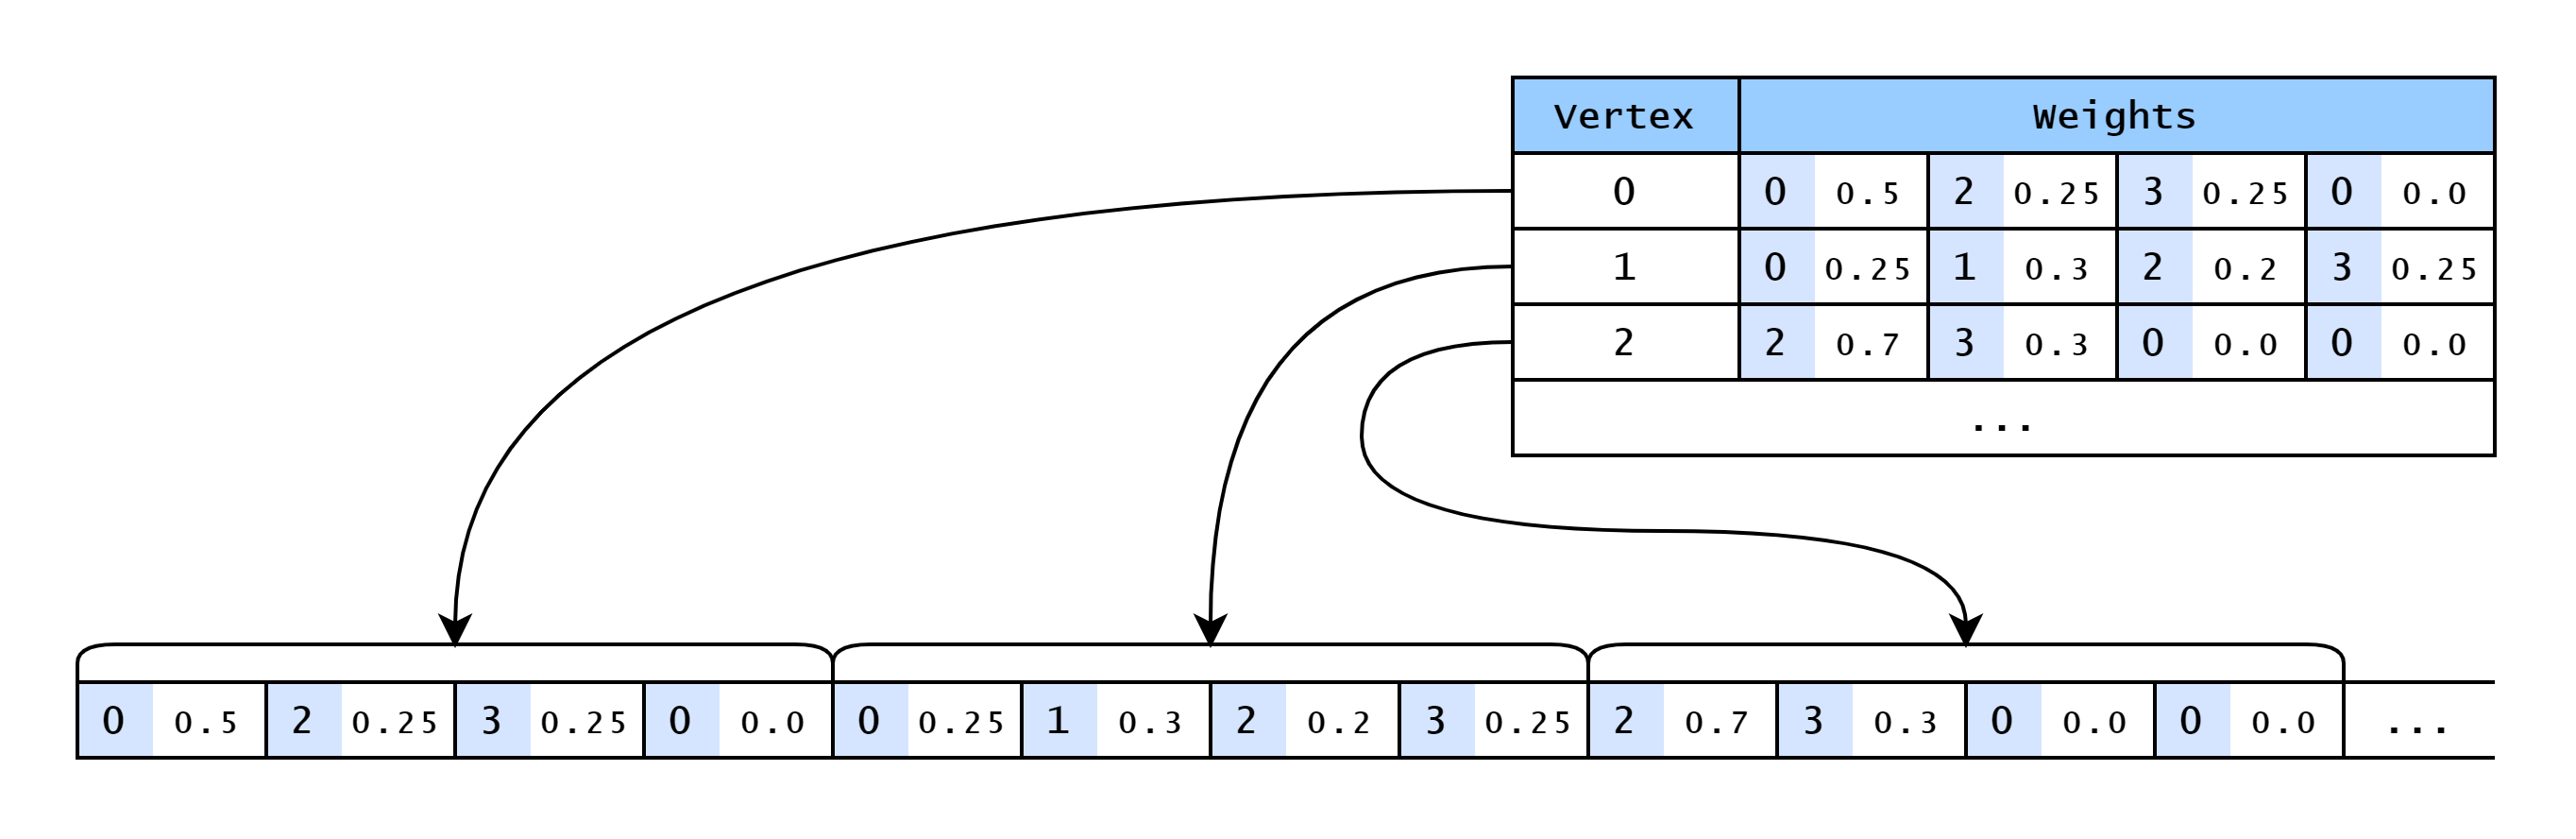
\includegraphics[width=1.0\textwidth]{figures/joint_weights.png}
    \caption{Joint weight layout}
    \label{fig:joint-weights}
\end{figure}

Each \code{Primitive} also contains \code{positions\_cpu} and \code{joint\_weights\_cpu}, which store the same data in \code{std::vector}s for easier CPU access during skinning.

A \code{Mesh} can optionally contain a \code{Blas}, created for the static mesh, i.e., a node uses the mesh without a skin.

\subsubsection{The \code{Skin} class}

The \code{Skin} class closely mirrors the glTF skin object. It stores an array of \code{Node}s representing the joints in the skeleton and an array of inverse bind matrices, with one entry per joint.

\subsubsection{The \code{Node} class}

The \code{Node} class represents a glTF node. The node transform can be stored as a matrix or as separate translation, rotation, and scale values. To model this, we use the \code{RawTransform} struct, which contains translation, rotation, and scale, and the \code{NodeTransform} struct, which stores the local transform (see \autoref{fig:node-transform}).

\begin{figure}[H]
\begin{lstlisting}[language=C++]
struct NodeTransform {
    bool raw;
    union {
        glm::mat4 matrix;
        RawTransform raw;
    } transform;
}
\end{lstlisting}
\caption{Structure used to store local transform of a node}
\label{fig:node-transform}
\end{figure}

The union \code{transform} stores either a \code{glm::mat4} or a \code{RawTransform}. The boolean \code{raw} determines how the union should be interpreted: if \code{raw} is \code{true}, it contains a raw transform; otherwise, it contains a matrix. The node also stores a global transform as a 4x4 matrix, which is only valid after calling \code{Node::update\_global\_transform}.

A node stores an array of child nodes and optionally a \code{Mesh}. If a mesh is present, the node stores a \code{Blas} and must generate a \code{TlasInstance} referencing its \code{Blas} when building the acceleration structure. After the first build, the node stores the index of its \code{TlasInstance}, used for updates. If the node has no \code{Skin}, its \code{Blas} is the same as the mesh's \code{Blas}.

If the node contains a \code{Skin}, it stores an array of sub-buffers for dynamic positions, which store vertex positions after skinning. This array contains one element for every primitive in the node's mesh. Each sub-buffer matches the size of the corresponding static positions sub-buffer. In this case, the node's \code{Blas} is dynamic and updated with the node's \code{dynamic\_positions}, rather than referencing the mesh's static \code{Blas}.

\subsubsection{The \code{Animation} class}

The \code{Animation} class represents a glTF animation. It contains an array of \code{AnimationSampler}s, each referencing the node it modifies and implementing a virtual \code{apply\_for} function. This function samples a value at a given time and applies it to a node's transform. Three subclasses of \code{AnimationSampler} override \code{apply\_for}:

\begin{itemize}
    \item \code{TranslationSampler}: samples a 3D vector and sets the node's translation.
    \item \code{RotationSampler}: samples a quaternion and sets the node's rotation.
    \item \code{ScaleSampler}: samples a 3D vector and sets the node's scale.
\end{itemize}

The animation itself also implements \code{apply\_for}, iterating over all channels and applying them at a given time.

\subsubsection{Buffers and Sub-Buffers}

glTF uses buffers, buffer views, and accessors. We do not use the glTF buffers directly; instead, we reorganize the data for convenience. Accessors may point to interleaved or sparse data, and component types may differ. To obtain sequential, fixed-type arrays, we use the cgltf functions \code{cgltf\_accessor\_unpack\_floats} for floats and \code{cgltf\_accessor\_unpack\_indices} for unsigned integers. These functions read an accessor's elements and store them in a sequence of the desired type in a target buffer.

We create separate buffers for vertex indices, joint weights, static positions, and dynamic positions. Attributes reference a sub-section of a buffer using a sub-buffer. Each sub-buffer holds a reference to the buffer (\code{ptr::Shared<Buffer>}), an offset, and a length. The element type is implied by the variable storing the sub-buffer (e.g., \code{positions} in a \code{Mesh} stores \code{vec3}s).

\autoref{fig:scene-buffers} illustrates sub-buffer usage:

\begin{figure}[H]
    \centering
    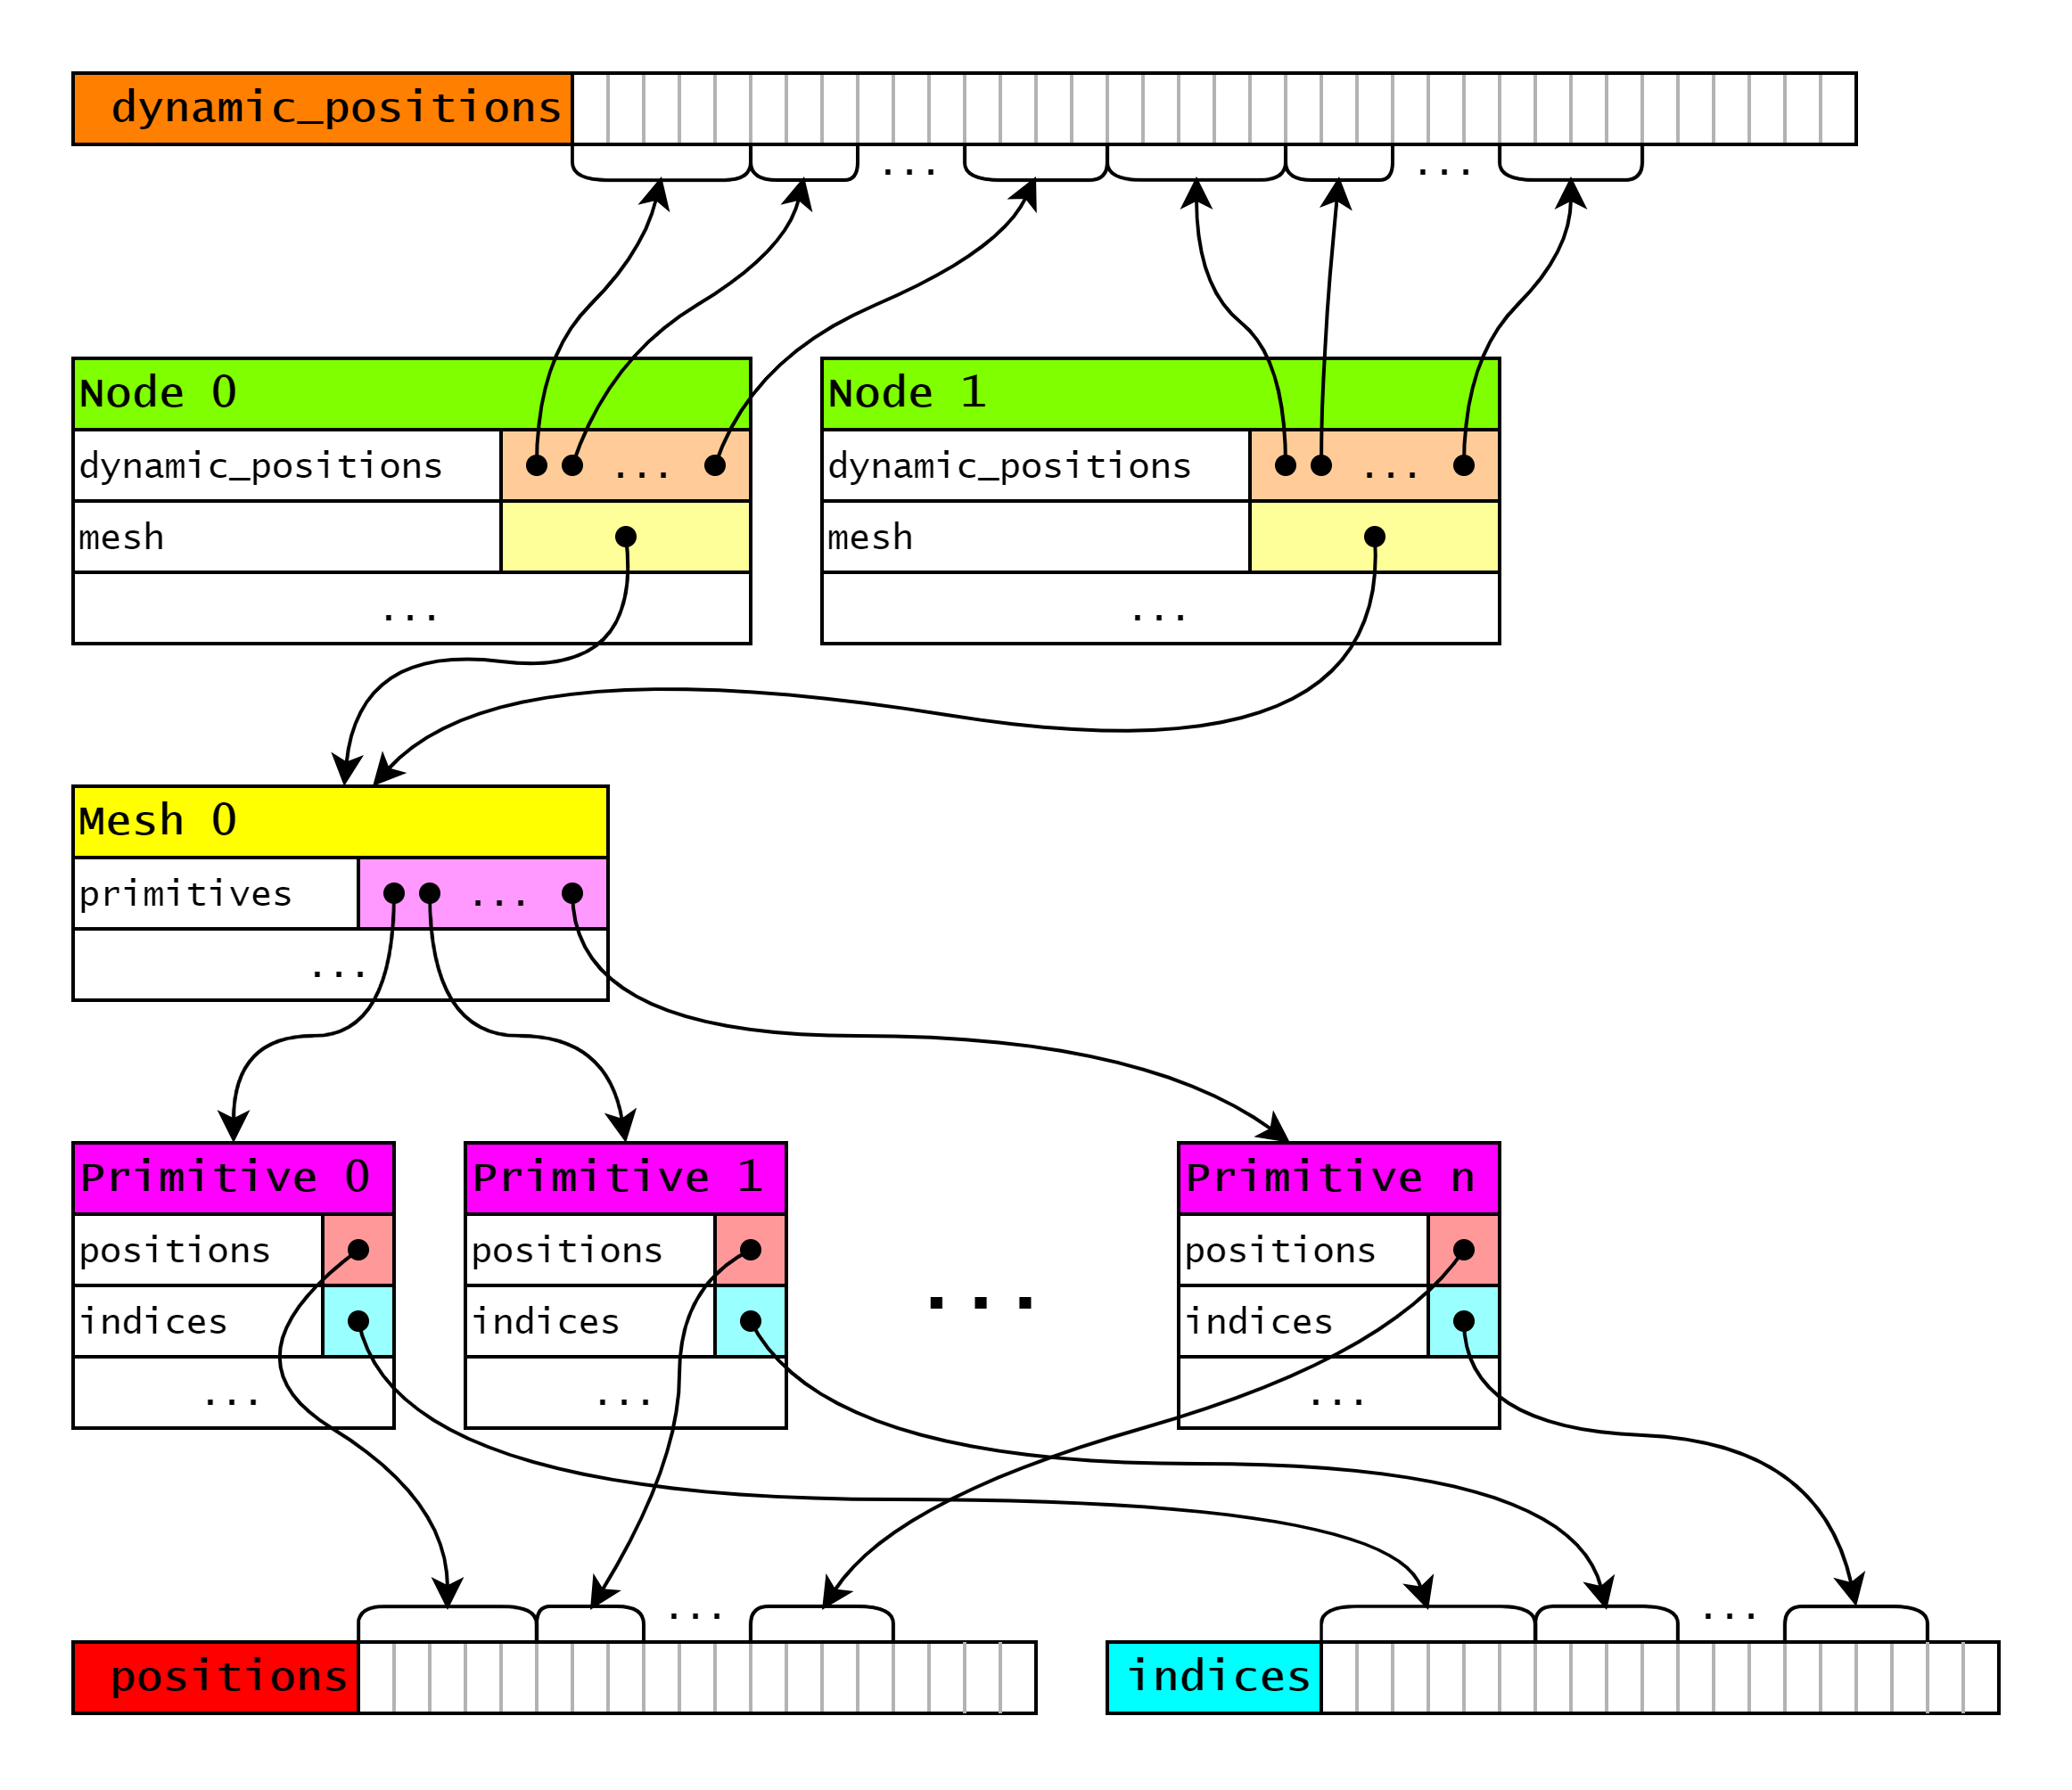
\includegraphics[width=1.0\textwidth]{figures/scene_buffers.png}
    \caption{Usage of sub-buffers in a scene}
    \label{fig:scene-buffers}
\end{figure}

The example in \autoref{fig:scene-buffers} shows two nodes (\code{Node 0} and \code{Node 1}), which reference the same mesh (\code{Mesh 0}) and therefore share static positions and indices. However, since each node may use a different skin, each stores its own \code{dynamic\_positions} sub-buffer matching the size of the static positions. For simplicity, joint weights are not shown in the example.

\subsection{Updating a Scene}\label{subsec:updating-a-scene}

Since scenes are dynamic, they must be updated after calling \code{Animation::apply\_for}. Updating occurs in three steps:

\begin{enumerate}
    \item Update global transforms for all nodes.
    \item Skin all animated models.
    \item Update the acceleration structure.
\end{enumerate}

The order is important, but we separate the steps to allow alternative implementations (e.g., CPU or GPU skinning, rebuilding or refitting the acceleration structure).

\subsubsection{Updating Global Transform}

\code{Node::update\_global\_transform} updates a node's global transform. It takes an optional \code{glm::mat4} parent transform, defaulting to the identity matrix.

Pseudo-code:

\begin{algorithm}[H]

\caption{Pseudo code for updating the global transform}\label{alg:global-transform}
    
\begin{algorithmic}[1]
    \Function{update\_global\_transform}{node, parent\_transform}
        \State node.global\_transform $\gets$ parent\_transform $\times$ node.transform
        \ForAll{child in node.children}
            \State update\_global\_transform(child, global\_transform)
        \EndFor
    \EndFunction
\end{algorithmic}

\end{algorithm}

The global transform is computed by pre-multiplying the parent transform with the node's local transform. This function is called recursively for all child nodes.

\subsubsection{Skinning}

Skinning applies skeleton deformation to a mesh. The first step in the skinning process is calculating the joint matrices:

\begin{algorithm}[H]

\caption{Calculating joint matrices}\label{alg:joint-matrices}

\begin{algorithmic}[1]
    \For{$i \gets 0$ to joints.count  - $1$}
        \State joint\_matrices[$i$] =  $inverse$(node.global\_transform)
        
        $\times$ joints[$i$].global\_transform
        
        $\times$ inverse\_bind\_matrices[$i$]
    \EndFor
\end{algorithmic}

\end{algorithm}

The mesh is then skinned:

\begin{algorithm}[H]

\caption{Skinning a model}\label{alg:skinning}

\begin{algorithmic}[1]
    \For{$j \gets 0$ to (positions.count $-1$)}
        \State matrix $\gets$ $0_{4 \times 4}$
        \ForAll{joint\_weight in joint\_weights[$i$]}
            \State matrix $\gets$ matrix + joint\_weight.weight $\times$ joint\_matrices[joint\_weight.index]
        \EndFor

        \State position $\gets$ matrix $\times$ position
        \State dynamic\_positions[$i$] $\gets$ matrix $\times$ positions[i]
    \EndFor
\end{algorithmic}

\end{algorithm}

This algorithm uses \textbf{Linear Blend Skinning}, which is the standard skinning technique to its simplicity and efficiency~\parencite{linear-blend-skinning}. For each vertex, we compute a weighted sum of joint matrices and apply it to the vertex position.

Our application offers two implementations:

\begin{itemize}
    \item \textbf{CPU skinning}
    
    Reads positions from a primitives \code{positions} sub-buffer, runs the algorithm on the CPU, and writes results to the respective \code{dynamic\_positions}.

    \item \textbf{GPU skinning}
    
    Uses a vertex shader to process each vertex and store results in a storage buffer. Rasterization is disabled, stopping the pipeline after the vertex shader. A compute shader could also be used, but this approach uses the rasterization pipeline already implemented in our application.

\end{itemize}

\subsubsection{Updating the acceleration structure}

\begin{algorithm}[H]

\caption{Updating acceleration structure}\label{alg:acceleration-structure-update}

\begin{algorithmic}[1]
    \Function{update\_acceleration\_structure}{scene}
        \State node\_iterator = get\_node\_iterator(scene)
        \State tlas\_instances = get\_instances(scene.tlas)
        \ForAll{node in node\_iterator}
            \If{has\_blas(node)}
                \If{is\_dynamic(node.blas)}
                    \State update(node.blas)
                \EndIf
                \State update\_tlas\_instance(tlas, node)
            \EndIf
        \EndFor
        \State update(scene.tlas)
    \EndFunction
\end{algorithmic}

\end{algorithm}

There is no single \code{Scene::update\_acceleration\_structures} function. Instead, our application offers two functions:

\begin{itemize}
    \item \code{Scene::rebuild\_acceleration\_structures}
    \item \code{Scene::refit\_acceleration\_structures}
\end{itemize}

Both follow the same algorithm shown in Algorithm \ref{alg:acceleration-structure-update}; the only difference is whether the acceleration structures are rebuilt from scratch or only refitted.

\pagebreak